%----------------------------------------------------------------------------------------
%	PACKAGES AND DOCUMENT CONFIGURATIONS
%----------------------------------------------------------------------------------------

\documentclass[12pt,a4paper]{article}

\usepackage[version=3]{mhchem} % Package for chemical equation typesetting
\usepackage{siunitx} % Provides the \SI{}{} and \si{} command for typesetting SI units
\usepackage{graphicx} % Required for the inclusion of images
\usepackage{natbib} % Required to change bibliography style to APA
\usepackage{amsmath} % Required for some math elements 
\usepackage{geometry}
\usepackage{enumerate}
\usepackage{float}
\usepackage{subfigure}
\usepackage{pdfpages}
\usepackage{siunitx}
\usepackage{fancyhdr}
\usepackage{textcomp}
\usepackage{gensymb}
\usepackage{longtable}

\includepdfset{pagecommand={\thispagestyle{fancy}}}%page number for pdf

\renewcommand{\labelenumi}{\alph{enumi}.} % Make numbering in the enumerate environment by letter rather than number (e.g. section 6)
\geometry{left=2cm,right=2cm,top=3cm,bottom=3cm}

%\usepackage{times} % Uncomment to use the Times New Roman font

%----------------------------------------------------------------------------------------
%	DOCUMENT INFORMATION
%----------------------------------------------------------------------------------------


\begin{document}

\begin{center}
~\\
\rule[0mm]{400pt}{0.5pt}
\Large{ \textsc{\newline\\UM-SJTU Joint Institute\\Physics Laboratory\\(Vp241)\\}}
\rule[0mm]{400pt}{0.5pt}
\Large{ \textsc{\newline\newline\newline\newline\newline\newline\\
Laboratory Report\\}}
\Large{\textsc{ \\ Exercise 5  \\ RC, RL, and RLC Circuits} }

\end{center}

\begin{description}
    \item[] 
    \item[] 
    \item[] 
    \item[] 
    \item[] 
    \item[]
    \item[]\qquad \qquad Name: Han Yibei \qquad ID:519370910123   \qquad    Group:11\\
    \item[]\qquad \qquad Date: \today
\end{description}

\newpage

%----------------------------------------------------------------------------------------
%	SECTION 1
%----------------------------------------------------------------------------------------
\section{Abstract}
This experiment is study the time constant, half period, the phase difference and current amplitude in circuits containing source, resistors, capacitors and resistors. Through the experiment, we could found that the time constant for RC, RL, and RLC are 11.2530$\pm0.0014$, 95.218$\pm0.014$, 30.952$\pm0.06~[\times 10^{-6}s]$. And their theoretical values are 10.0686, 98.921, 31.560 $[\times10^{-6}s]$ with relative error 11.76\%, -3.74\% and -1.93\%. In RLC resonant circuits, the tested resonant frequency is 5040.000$\pm0.001$Hz, with relative error -0.06\% to theoretical 5043$\pm3$Hz. The figure of experimental $\varphi \text{ vs }\frac{f}{f_0}$ verifies the theoretical one. Calculations, figures and plots are used to analyze the experiment.

\section{Introduction}
\subsection{Motivation}
This experiment help the understading of RC, RL and RLC circuits and their characteristics, especially the damping situations. The RLC circuit is the foundation of engineering. Through the learning we can do better in circuit design. 

\subsection{Theoretical Background}
\subsubsection{Transient Processes in RC, RL, RLC Series Circuits}
\textbf{\qquad RC Series Circuits} \par
In an RC circuit, the transient process include the capicitor's charge and dischargr. Fig.\ref{rccir} is an RC series circuit.
\begin{figure}[H]
    \centering
    \includegraphics[width=6cm]{rccir.png}
    \caption{RC series circuit    [1]}
    \label{rccir}
\end{figure}

At the first half period of voltage $U(t) =\mathcal{E}$ and the capacitor charges. In the second half period, voltage is zero, and the capacitor discharges. The loop equation (KVL) for the charging process is

\begin{equation}
    Rc\frac{dU_c}{dt}+U_c=\mathcal{E}~~~~\text{[1]}
\end{equation}

with $U_C(t = 0) = 0$, the solution of Eq.1 is
$$U_c=\mathcal{E}(1-e^{-\frac{t}{RC}})\text{ and }U_R=iR=\mathcal{E}e^{-\frac{t}{RC}}~~~~\text{[1]}$$

The capacitor $U_C$ increases with time t, also the voltage $U_R$ decreases. The curves of $U$(t), $U_c$(t), and $U_R$(t) are in Fig.\ref{rcfig}.

For the second half period:

\begin{equation}
    Rc\frac{dU_c}{dt}+U_c=0~~~~\text{[1]}
\end{equation}

With $U_C(t = 0) = \mathcal{E}$, the solution of Eq.2 is
$$U_c=\mathcal{E}e^{-\frac{t}{RC}}\text{ and }U_R=iR=\mathcal{E}e^{-\frac{t}{RC}}~~~~\text{[1]}$$

where $U_C$ and $U_R$ decrease with time. $RC=\tau$ is the time constant.The half-life period $T_{1/2}$ is the time used for circuit to decrease half of its volatge.
$T_{1/2} = \tau ln 2 \approx 0.693 \tau$.


\begin{figure}[H]
    \centering
    \includegraphics[width=14cm]{rcfig.png}
    \caption{Charging/discharging curves for a RC series circuit    [1]}
    \label{rcfig}
\end{figure}

\textbf{\qquad RL Series Circuit}
As we did in RC series circuit
$$\tau=\frac{L}{R}\text{ and }T_{1/2}=\frac{L}{R}ln 2~~~~[1]$$

\textbf{\qquad RLC Series Circuit}
When applied voltage, the RLC circuit can be analyzed as:
\begin{equation}
    LC\frac{d^2U_C}{dt}+U_c=\mathcal{E}~~~~[1]
\end{equation}
We can find that:
\begin{equation}
    \beta=\frac{R}{2L}\text{ and }\omega_0=\frac{1}{\sqrt{LC}}~~~~[1]
\end{equation}
Expressing Eq.3 by Eq.4, we can get:
\begin{equation}
    \frac{d^2U_C}{dt^2}+2\beta\frac{dU_C}{dt}+{\omega_0}^2U_C={\omega_0}^2\mathcal{E}~~~~[1]
\end{equation}
We can find the initial value for the equation is:
\begin{equation}
    U_C(t=0)=0\text{ and }\frac{dU_C}{dt}|_{t=0}=0~~~~[1]
\end{equation}

The relation between $\beta$ and $\omega_0$ cause three regimes,
\begin{itemize}
    \item 	If $|\beta|<|{\omega_0}|$, it's underdamped. The solution is:
    $$U_C=\mathcal{E}-\mathcal{E} e^{-\beta t}(cos{\omega}t+\frac{\beta}{\omega}sin{\omega}t)\text{ and } \omega=\sqrt{{\omega_0}^2-\beta^2}~~~~[1]$$
    \item If $|\beta|>|{\omega_0}|
    $, it's overdamped. The solution is:
    $$U_C=\mathcal{E}-\frac{\mathcal{E}}{2\gamma}e^{-\beta t}\left[\left(\beta+\gamma\right)e^{\gamma t}-\left(\beta-\gamma\right)e^{-\gamma t}\right]\text{ and }\gamma=\sqrt{\beta^2-{\omega_0}^2}~~~~[1]$$
    \item If $|\beta|=|{\omega_0}|$, it's critically damped. The solution is:
    $$U_C=\mathcal{E}-\mathcal{E}(1+\beta t)e^{-\beta t}~~~~[1]$$
\end{itemize}

When the power source is removed ($\mathcal{E}$= 0). The discharging process is similar to charging process.
The voltage across the capacitor finally reach steady state. (Figure \ref{rlc})

\begin{figure}[H]
    \centering
    \includegraphics[width=12cm]{rlc.png} 
    \caption{Three different regimes of transient processes in an RLC series circuit    [1]}
    \label{rlc}
\end{figure}

\subsubsection{RC, RL Steady-State Circuits}
The phase change can be determined as: 
$$\varphi={tan}^{-1}{(}\frac{U_L}{U_R})={tan}^{-1}{(}\frac{\omega L}{R})~~~~[1]$$
$$\varphi={tan}^{-1}{(}-\frac{U_C}{U_R})={tan}^{-1}{(}-\frac{1}{\omega RC})~~~~[1]$$

\subsubsection{RLC Resonant Circuit}
\textbf{\qquad RLC Series Circuit}
Take I as a vector along the horizontal axis, the phase differences across the resistor, coil, and capacitor are
$$\varphi_R=0~~~~~~~~\varphi_L=\frac{\pi}{2}~~~~~~~~\varphi_C=-\frac{\pi}{2}~~~~[1]$$
\begin{figure}[H]
    \centering
    \includegraphics[width=9cm]{rlcseries.png}
    \caption{RLC series circuit    [1]}
    \label{rlcseries}
\end{figure}
The corresponding voltages are
$$U_R=IZ=IR~~~~~~~~U_L=IZ_L=I\omega L~~~~~~~~U_C=IZ_C=\frac{I}{\omega C}~~~~[1]$$
Their amplitudes are:
$$U=\sqrt{U^2_R+(U_L-U_C)^2}~~~~~~~~\text{or}~~~~~~~~U=I\sqrt{R^2+(\omega L-\frac{1}{\omega C})^2}~~~~[1]$$
The total impedance is:
$$Z=\sqrt{R^2+(\omega L-\frac{1}{\omega C})^2}~~~~[1]$$
with the total phase difference:
$$\varphi=tan^{-1}(\frac{U_L-U_C}{U_R})=tan^{-1}(\frac{\omega L-\frac{1}{\omega C}}{R})~~~~[1]$$

\textbf{\qquad Resonance}
The frequency that will cause resonant is:
$$\omega_0L=\frac{1}{\omega_0C}\longrightarrow\omega_0=\frac{1}{\sqrt{LC}}~~~~[1]$$ And the impedence now is smallest with amplitude $Z_0 = R$. When the current is $I_m = U=R$, its maximum. The resonance frequency is $$f_0=\frac{\omega_0}{2\pi}=\frac{1}{2\pi\sqrt{LC}}~~~~[1]$$
\begin{figure}[H]
    \centering
    \includegraphics[width=12cm]{rlcgeneral.png}
    \caption{The impedance, the current and the phase difference as functions of the frequency for an RLC series circuit (generic sketches)~~~~[1]}
    \label{rlcgeneral}
\end{figure}
Also, $\varphi=\varphi_u-\varphi_iall$. According to Equation, when $f < f_0$, $\varphi< 0$. The total voltage lag. The circuit is apacitive.\par 
When $f = f_0$, $\varphi= 0$. The voltages is equal. The circuit is resistive. \par
When $f > f_0$, $\varphi> 0$. The total voltage lead. The circuit is inductive.


\section{Discription of Experiment}
\subsection{Apparatus}
The measurement setup consists of the following main elements: "a signal generator, an oscilloscope, a digital multimeter, a wiring board, a resistor, a variable resistor, a capacitor, as well as an inductor."[1]
\begin{figure}[H]
    \centering
    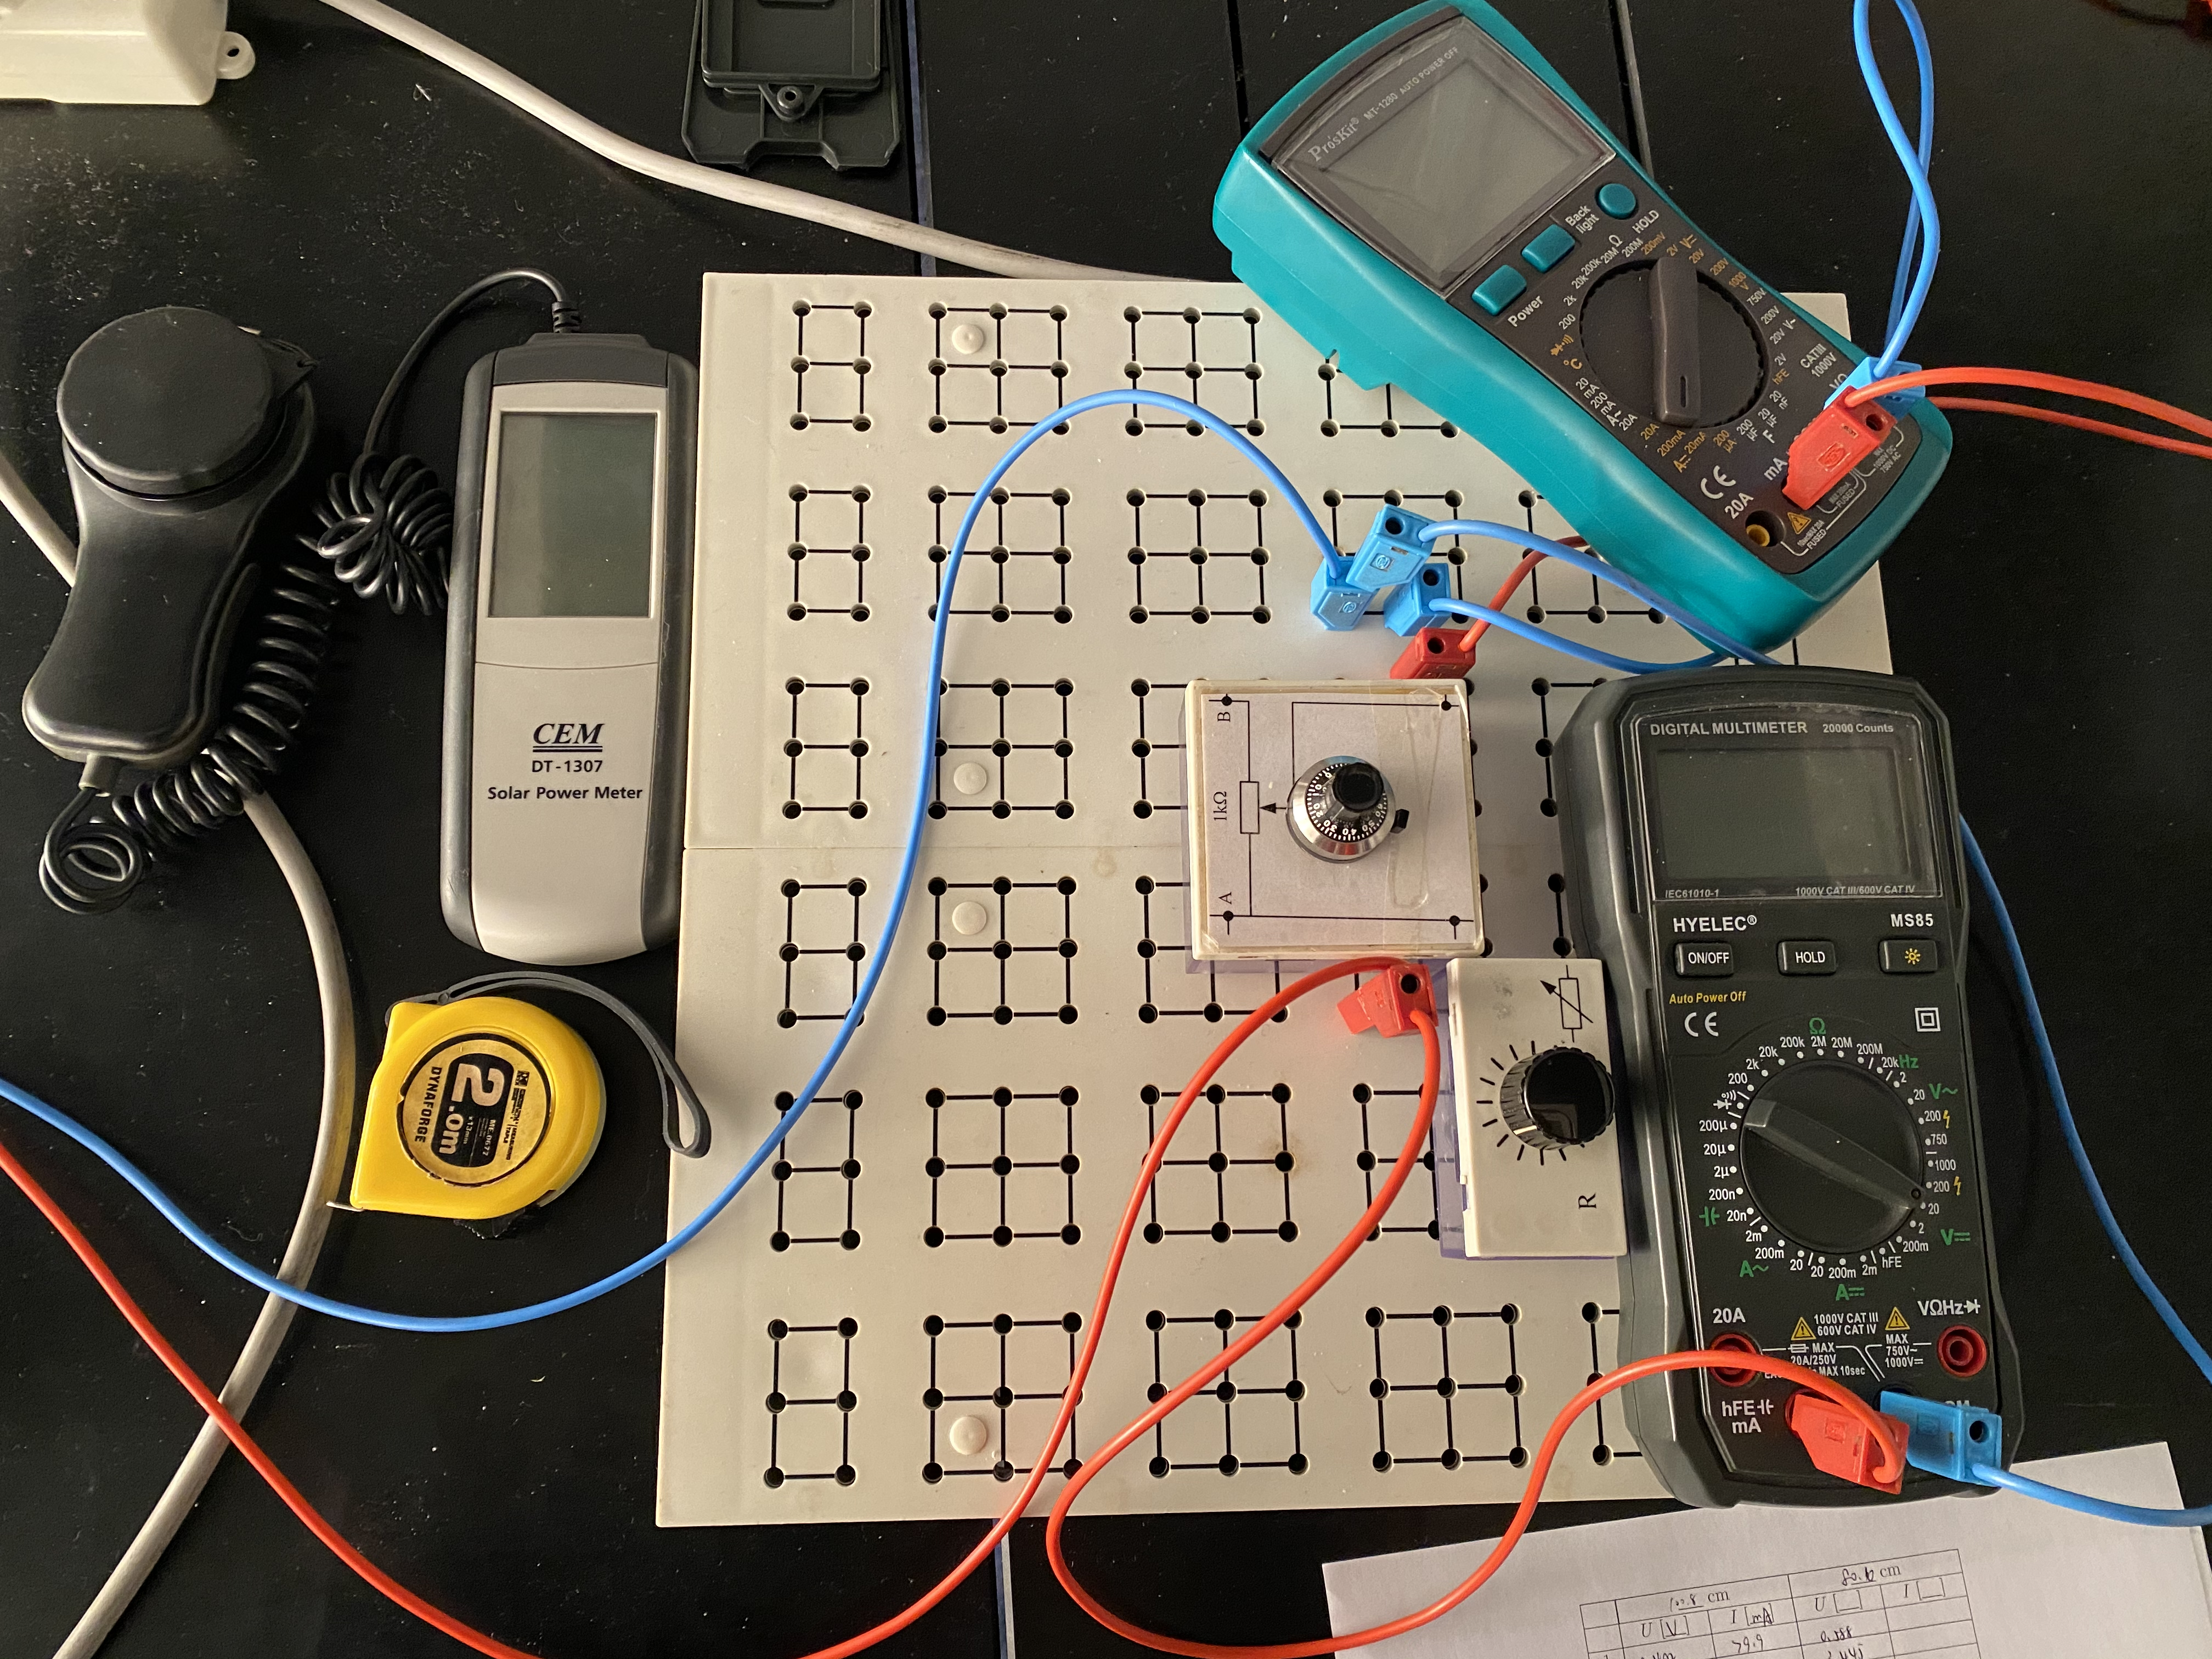
\includegraphics[width=9cm]{apparatus.jpg}
    \caption{Apparatus}
\end{figure}

\subsection{Device Information}
The information of each measurement device is shown in Table \ref{information}.

\begin{table}[H]
    \centering
    \begin{tabular}{|c|c|}
    \hline
    apparatus & uncertainty \\ \hline
    Signal generator & $\pm 0.001Hz/\pm 0.001 Vpp$ \\ \hline
    Cursor(time) & $\pm 0.01/0.001\mu s$\\ \hline
    Cursor(amplitude) & $\pm 0.02/0.002 Vpp$\\ \hline
    Multimeter(resistance)  & $\pm 0.01\Omega$\\ \hline
    Multimeter(capacitance) & $\pm 0.1nF$\\ \hline
    \end{tabular}
    \caption{Information of Each Measurement Device}
    \label{information}
\end{table}

\subsection{Measurement Procedure}
\subsubsection{RC, RL Series Circuit}
First, build the RC or RL circuit. Change the amplitude and frenquency of signal generator to an appropriate value. Use cursor function to measure $T_1/2$. Calculate the time constant and compare it with the theoretical value.

\subsubsection{RLC Series Circuit}
First, build the RLC circuit with the variable resistor. Observe the waveform when it is underdamping, critically damping, and overdamping. Adjust the variable resistor to make the circuit critically damping. We will have $\beta$T1/2 = 1.68. Then the time constant is $\tau= 1/\beta = T1/2/1.68$.

\subsubsection{RLC Resonant Circuit}
Change the RLC circuit above and use a resistor with fixed value. Change the frequency, then observe $U_R$. Then calculate the corresponding phase difference. Compare the experimental value to the theoretical one. Plot the graphs $I=I_m$ vs. $f=f_0$ and $\varphi vs. f=f0$. Also, estimate the resonance frequency and calculate the quality factor Q.

\subsubsection{Caution}
We do these to make uncertainty smaller:
\begin{itemize}
    \item Ground all the capacitors, inductors and resistors to the same point.
    \item Turn on power supply only after conpleting circuit
    \item Turn off power supply before changing the circuit
\end{itemize}


\section{Result}
\subsection{RC series circuit}
\begin{table}[H]
    \centering
    \begin{tabular}{|c|c|}
    \hline
    Quantities             & Value              \\ \hline
    R{[}$\Omega${]}        & 101.09$\pm$0.01    \\ \hline
    F{[}Hz{]}              & 1000.000$\pm$0.001 \\ \hline
    $\mathcal{E}${[}Vpp{]} & 4.000$\pm$0.001    \\ \hline
    C{[}nf{]}              & 99.6$\pm$0.1       \\ \hline
    T{[}$\mu$s{]}          & 7.800$\pm$0.001    \\ \hline
    \end{tabular}
    \caption{Measurement Data for RC circuit}
\end{table}
We than calculate the time constant $\tau_{exp}$:
$$\tau_{exp}=\frac{T_{1/2}}{ln2}=\frac{7.800}{ln2}=11.2530\pm0.0014\mu s=11.2530\pm0.0014 [\times 10^{-6}]s$$

Theoretically, the time constant ${\tau}_{theo}$ should be:
$${\tau}_{theo}=RC=101.09\times99.6\times 10^{-9}=10.0686[\times 10^{-6}]s$$

The relative error is:
$$u_r==\frac{\tau_{exp}-\tau_{theo}}{\tau_{theo}}=\frac{11.2530-10.0686}{10.0686}=11.76\%$$

\begin{figure}[H]
    \centering
    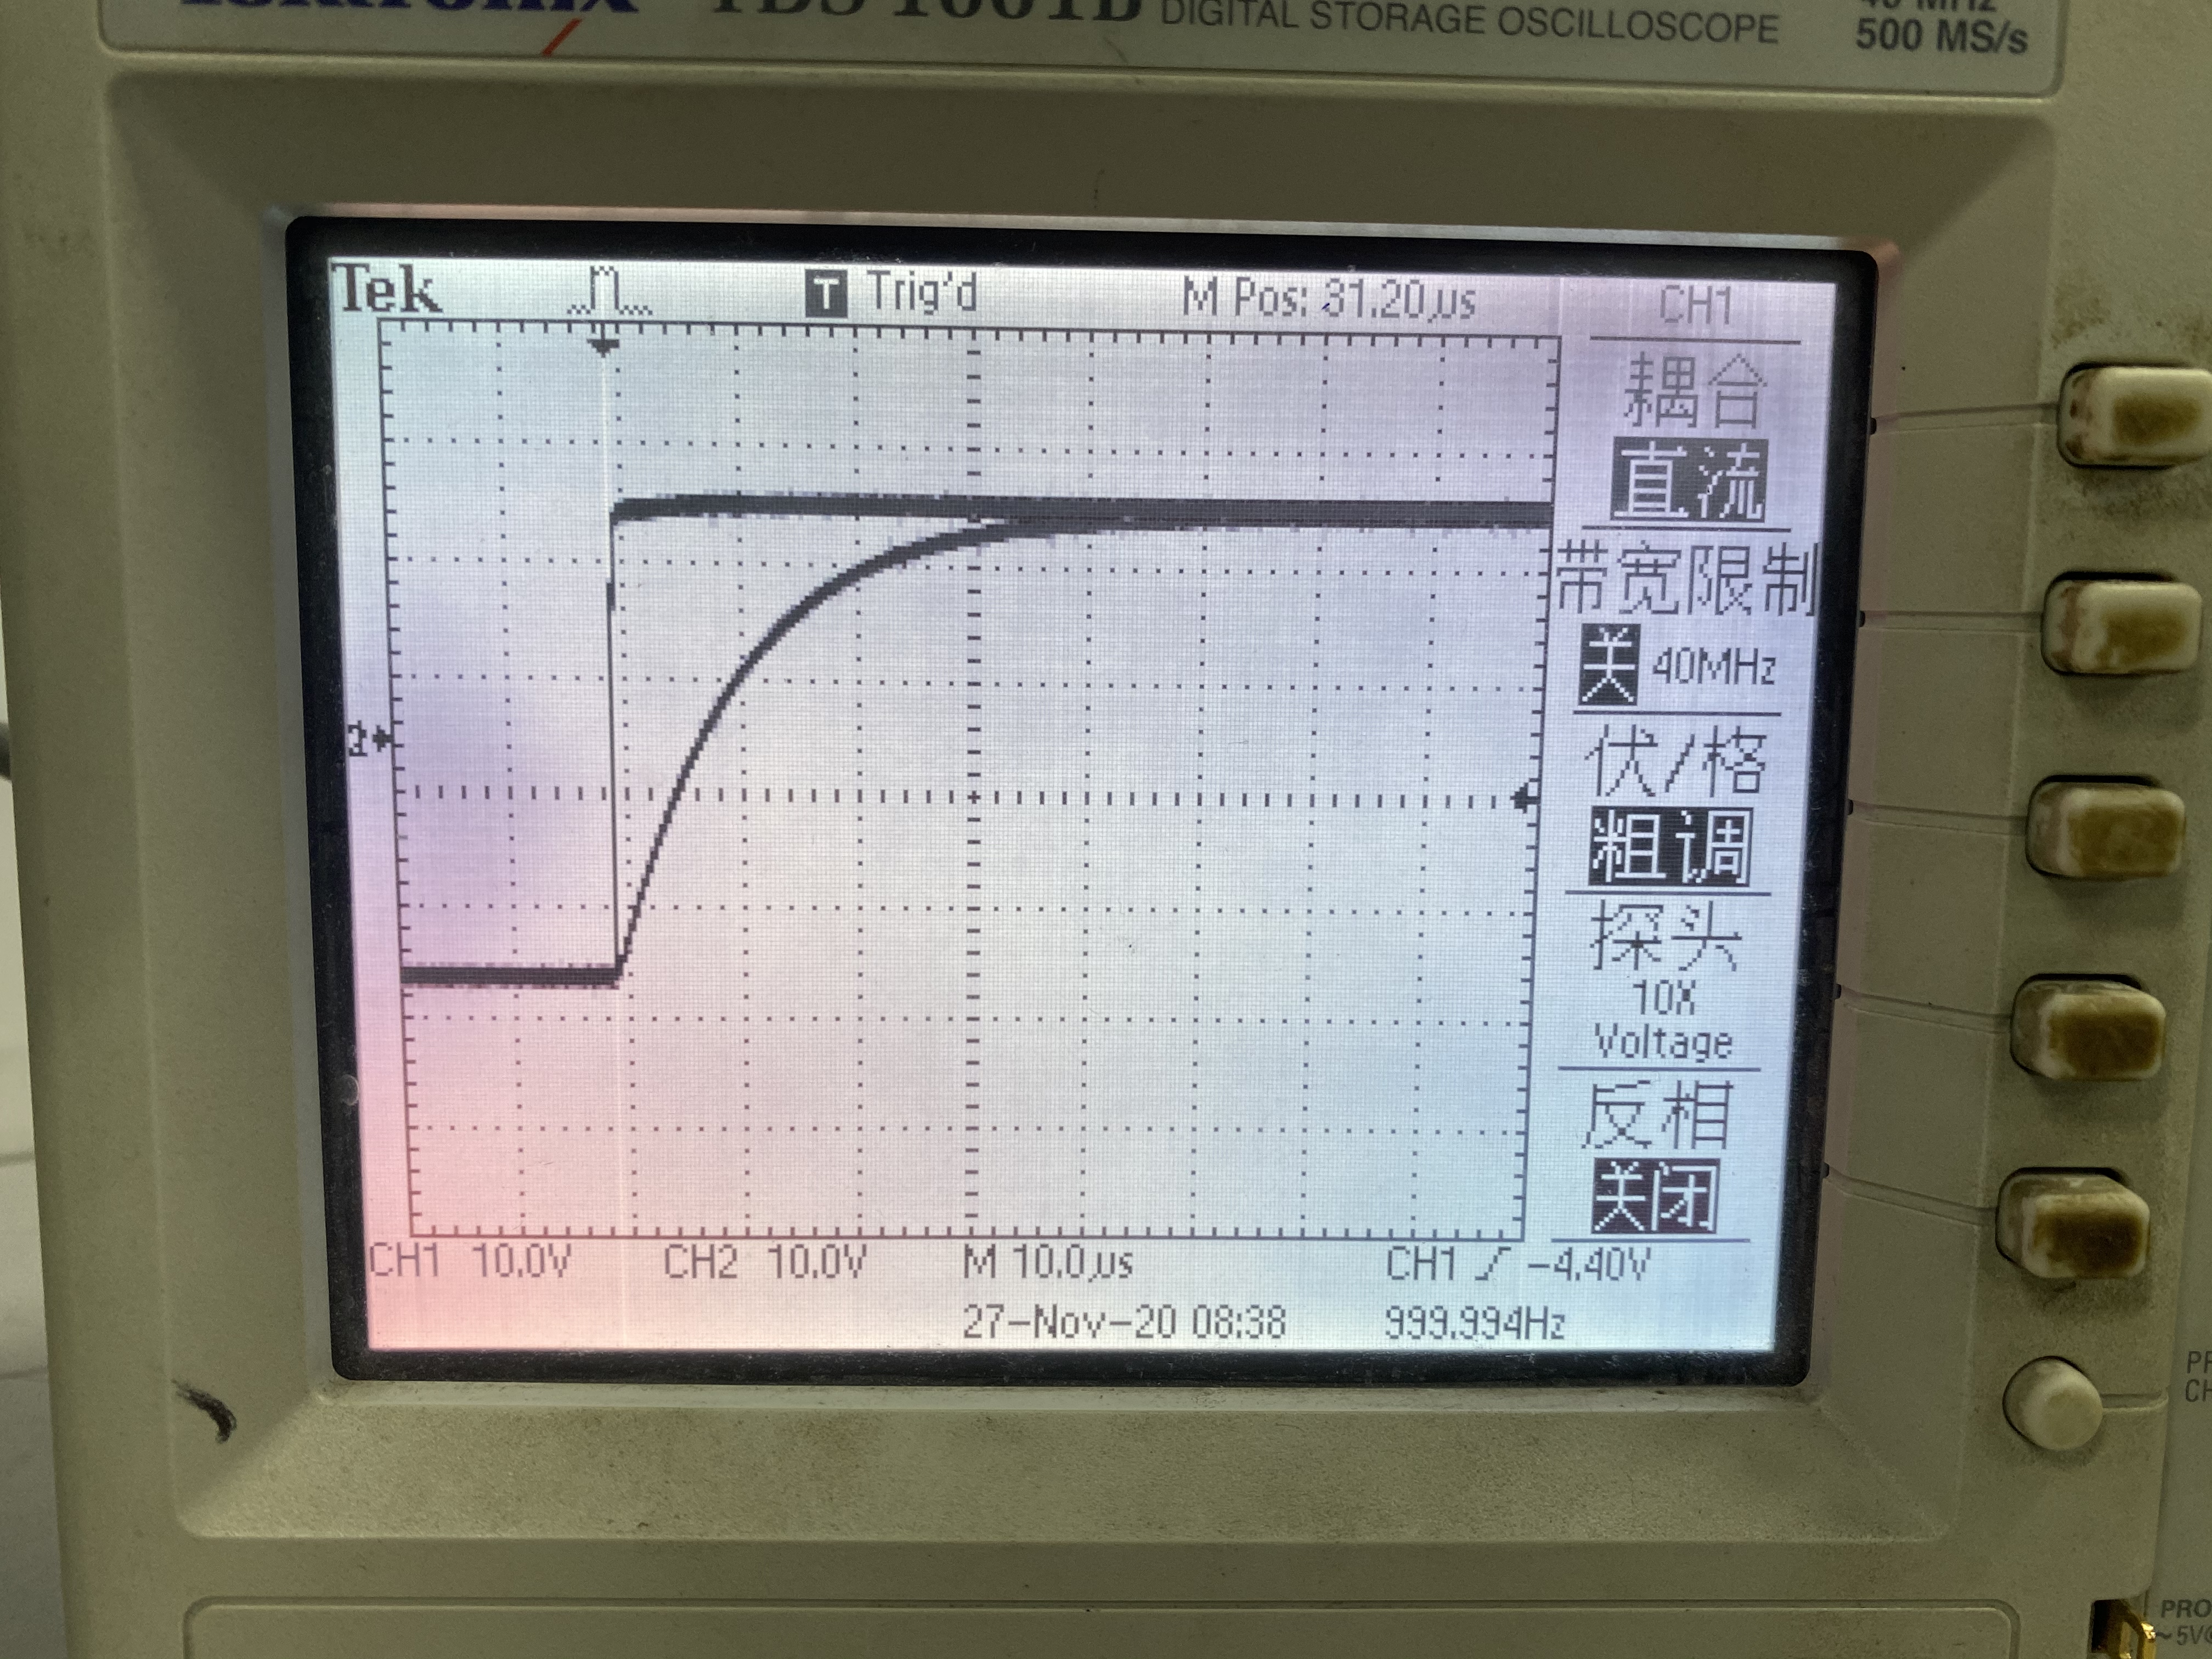
\includegraphics[width=7cm]{rcex.jpg}
    \caption{Waveform of RC circuit}
\end{figure}

\subsection{RL series circuit}
\begin{table}[H]
    \centering
    \begin{tabular}{|c|c|}
    \hline
    Quantities             & Value              \\ \hline
    R{[}$\Omega${]}        & 101.09$\pm$0.01    \\ \hline
    F{[}Hz{]}              & 500.000$\pm$0.001 \\ \hline
    $\mathcal{E}${[}Vpp{]} & 4.000$\pm$0.001    \\ \hline
    L{[}H{]}              & 0.01       \\ \hline
    T{[}$\mu$s{]}          & 66.00 $\pm$0.01    \\ \hline
    \end{tabular}
    \caption{Measurement Data for RC circuit}
\end{table}

\begin{figure}[H]
    \centering
    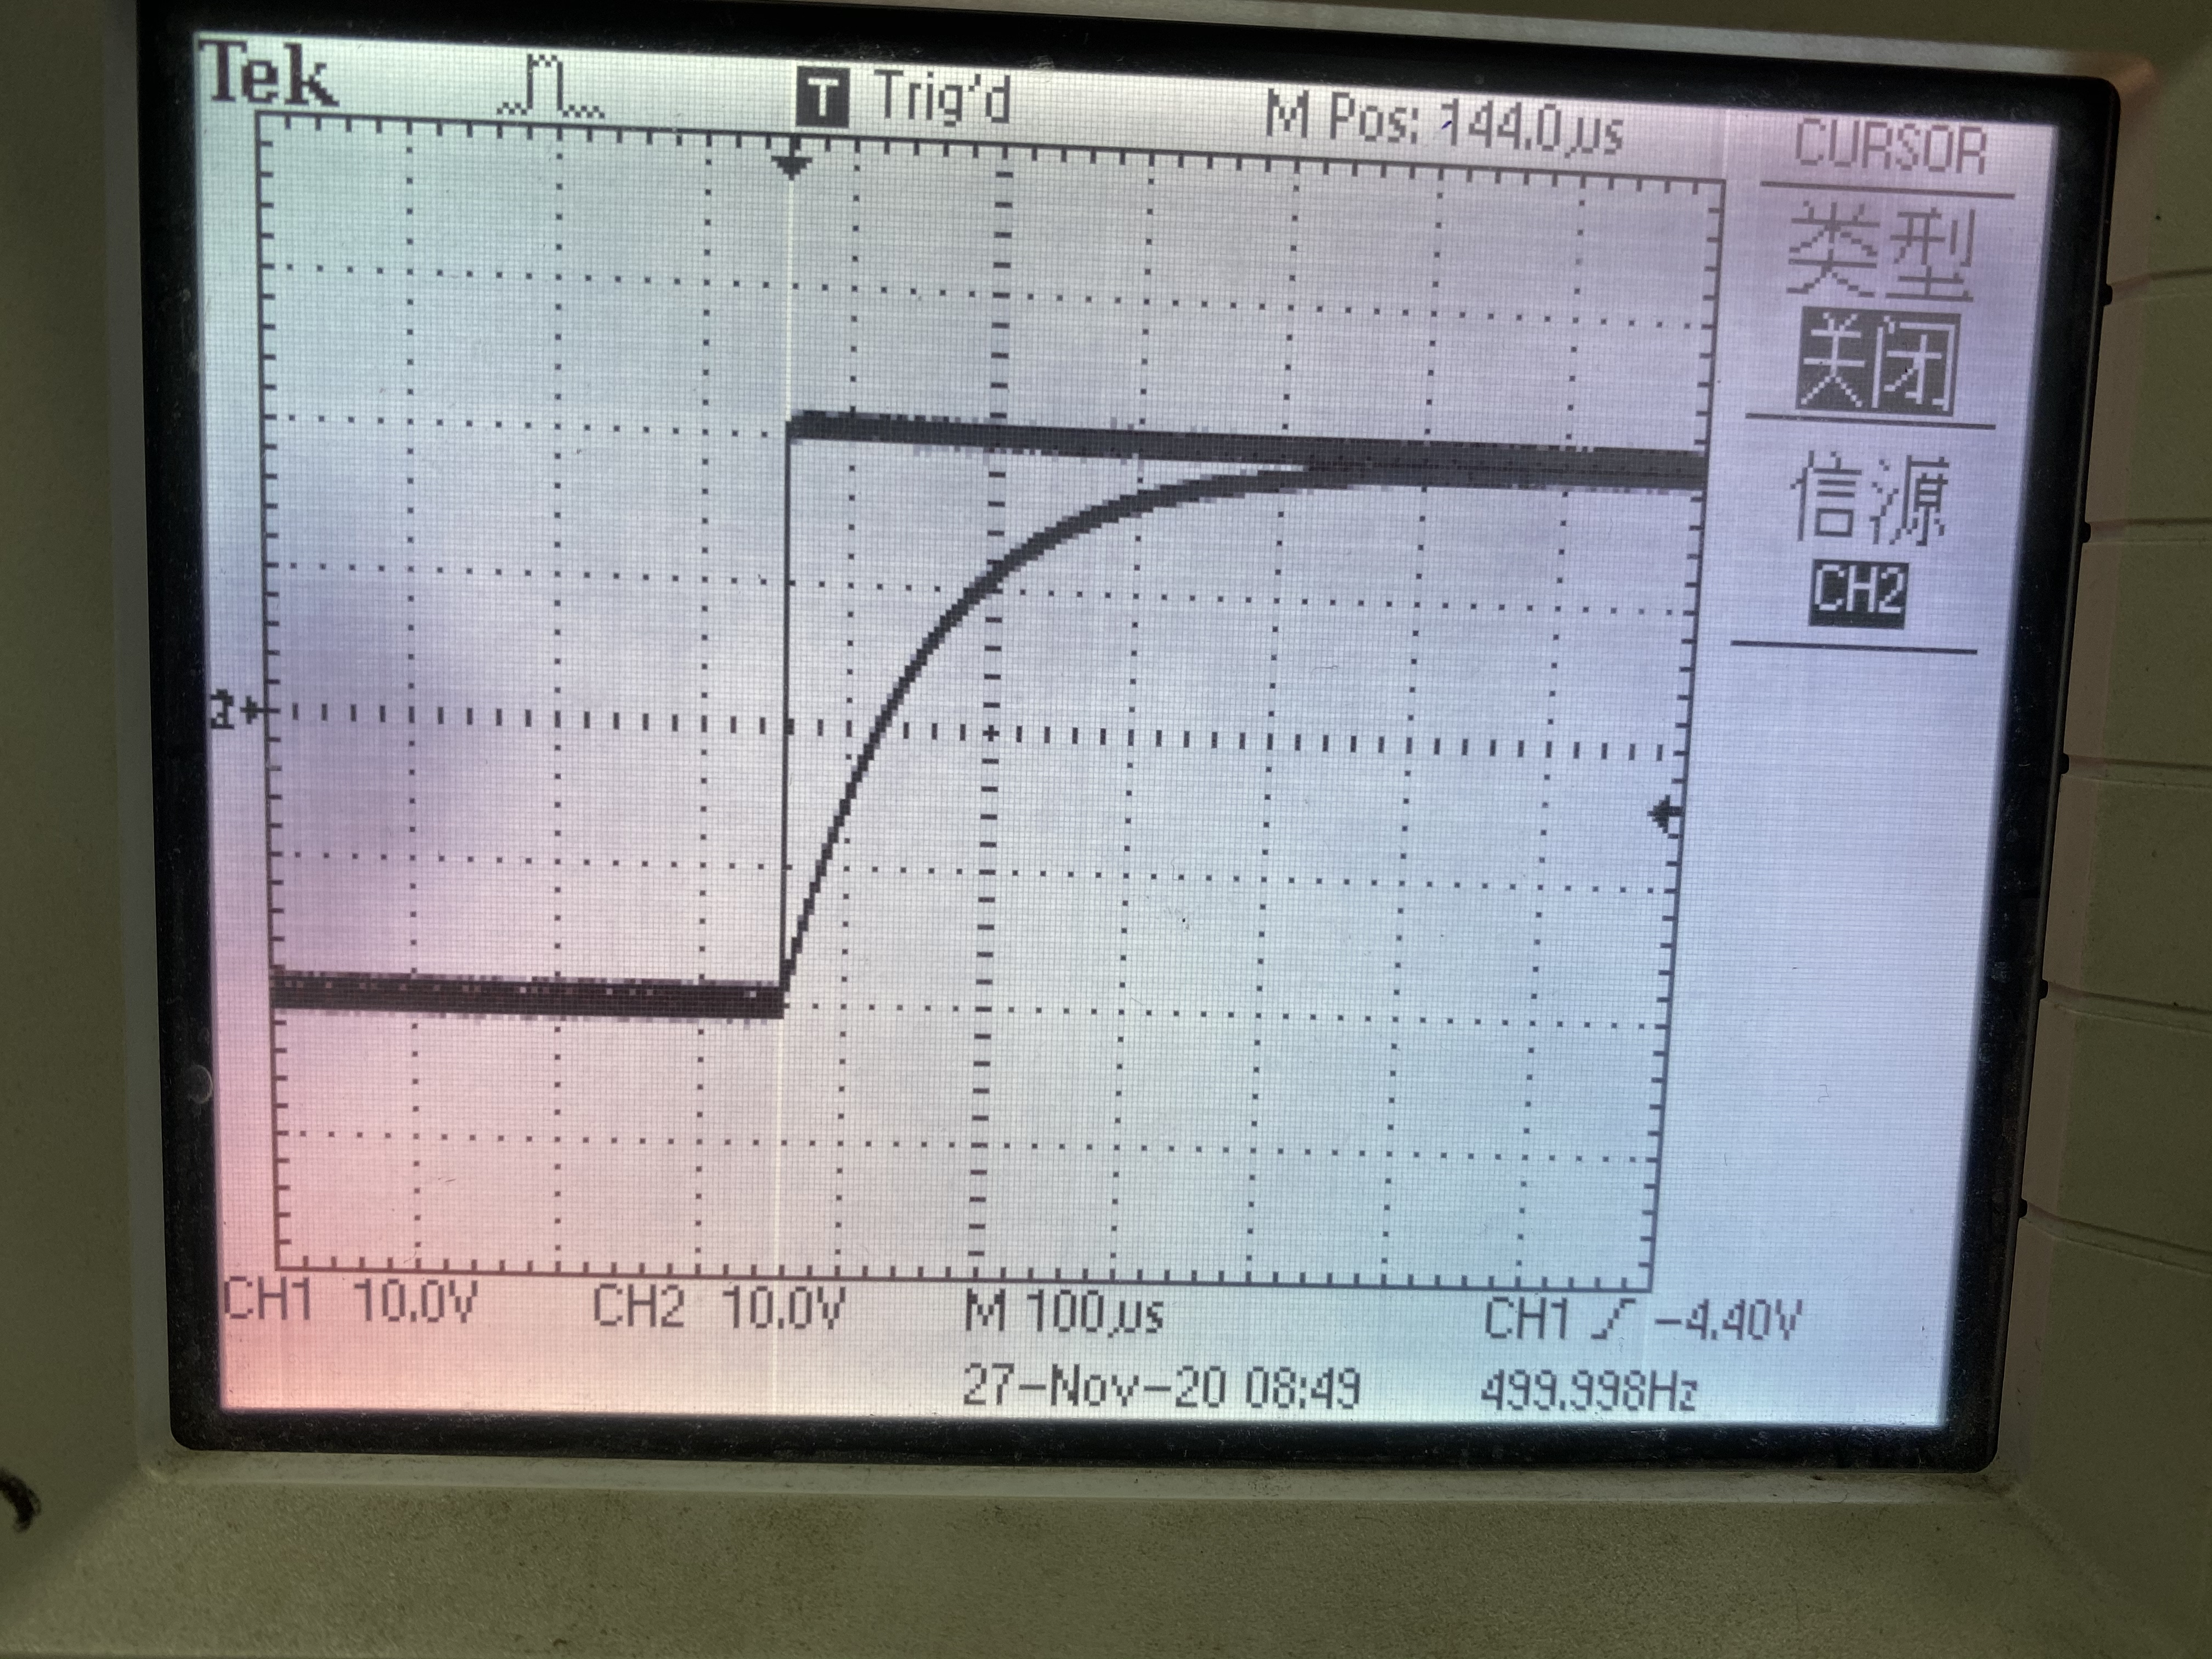
\includegraphics[width=7cm]{rlex.jpg}
    \caption{Waveform of RL circuit}
\end{figure}

We than calculate the time constant $\tau_{exp}$:
$$\tau_{exp}=\frac{T_{1/2}}{ln2}=\frac{7.800}{ln2}=95.218\pm0.014\mu s=95.218\pm0.014 [\times 10^{-6}]s$$

Theoretically, the time constant ${\tau}_{theo}$ should be:
$${\tau}_{theo}=\frac{L}{R}=\frac{0.01}{101.09}=98.921 [\times 10^{-6}]s$$

The relative error is:
$$u_r==\frac{\tau_{exp}-\tau_{theo}}{\tau_{theo}}=\frac{95.218-98.921}{98.921}=-3.74\%$$

\subsection{RLC series circuit}
\begin{table}[H]
    \centering
    \begin{tabular}{|c|c|}
    \hline
    Quantities             & Value              \\ \hline
    R{[}$\Omega${]}        & 101.09$\pm$0.01    \\ \hline
    F{[}Hz{]}              & 1000.000$\pm$0.001 \\ \hline
    $\mathcal{E}${[}Vpp{]} & 4.000$\pm$0.001    \\ \hline
    C{[}nf{]}              & 99.6$\pm$0.1       \\ \hline
    L{[}H{]}              & 0.01       \\ \hline
    T{[}$\mu$s{]}          & 52.00 $\pm$0.01    \\ \hline
    \end{tabular}
    \caption{Measurement Data for RLC circuit}
\end{table}

\begin{figure}[H]
    \begin{minipage}{0.49\linewidth}
        \centering
        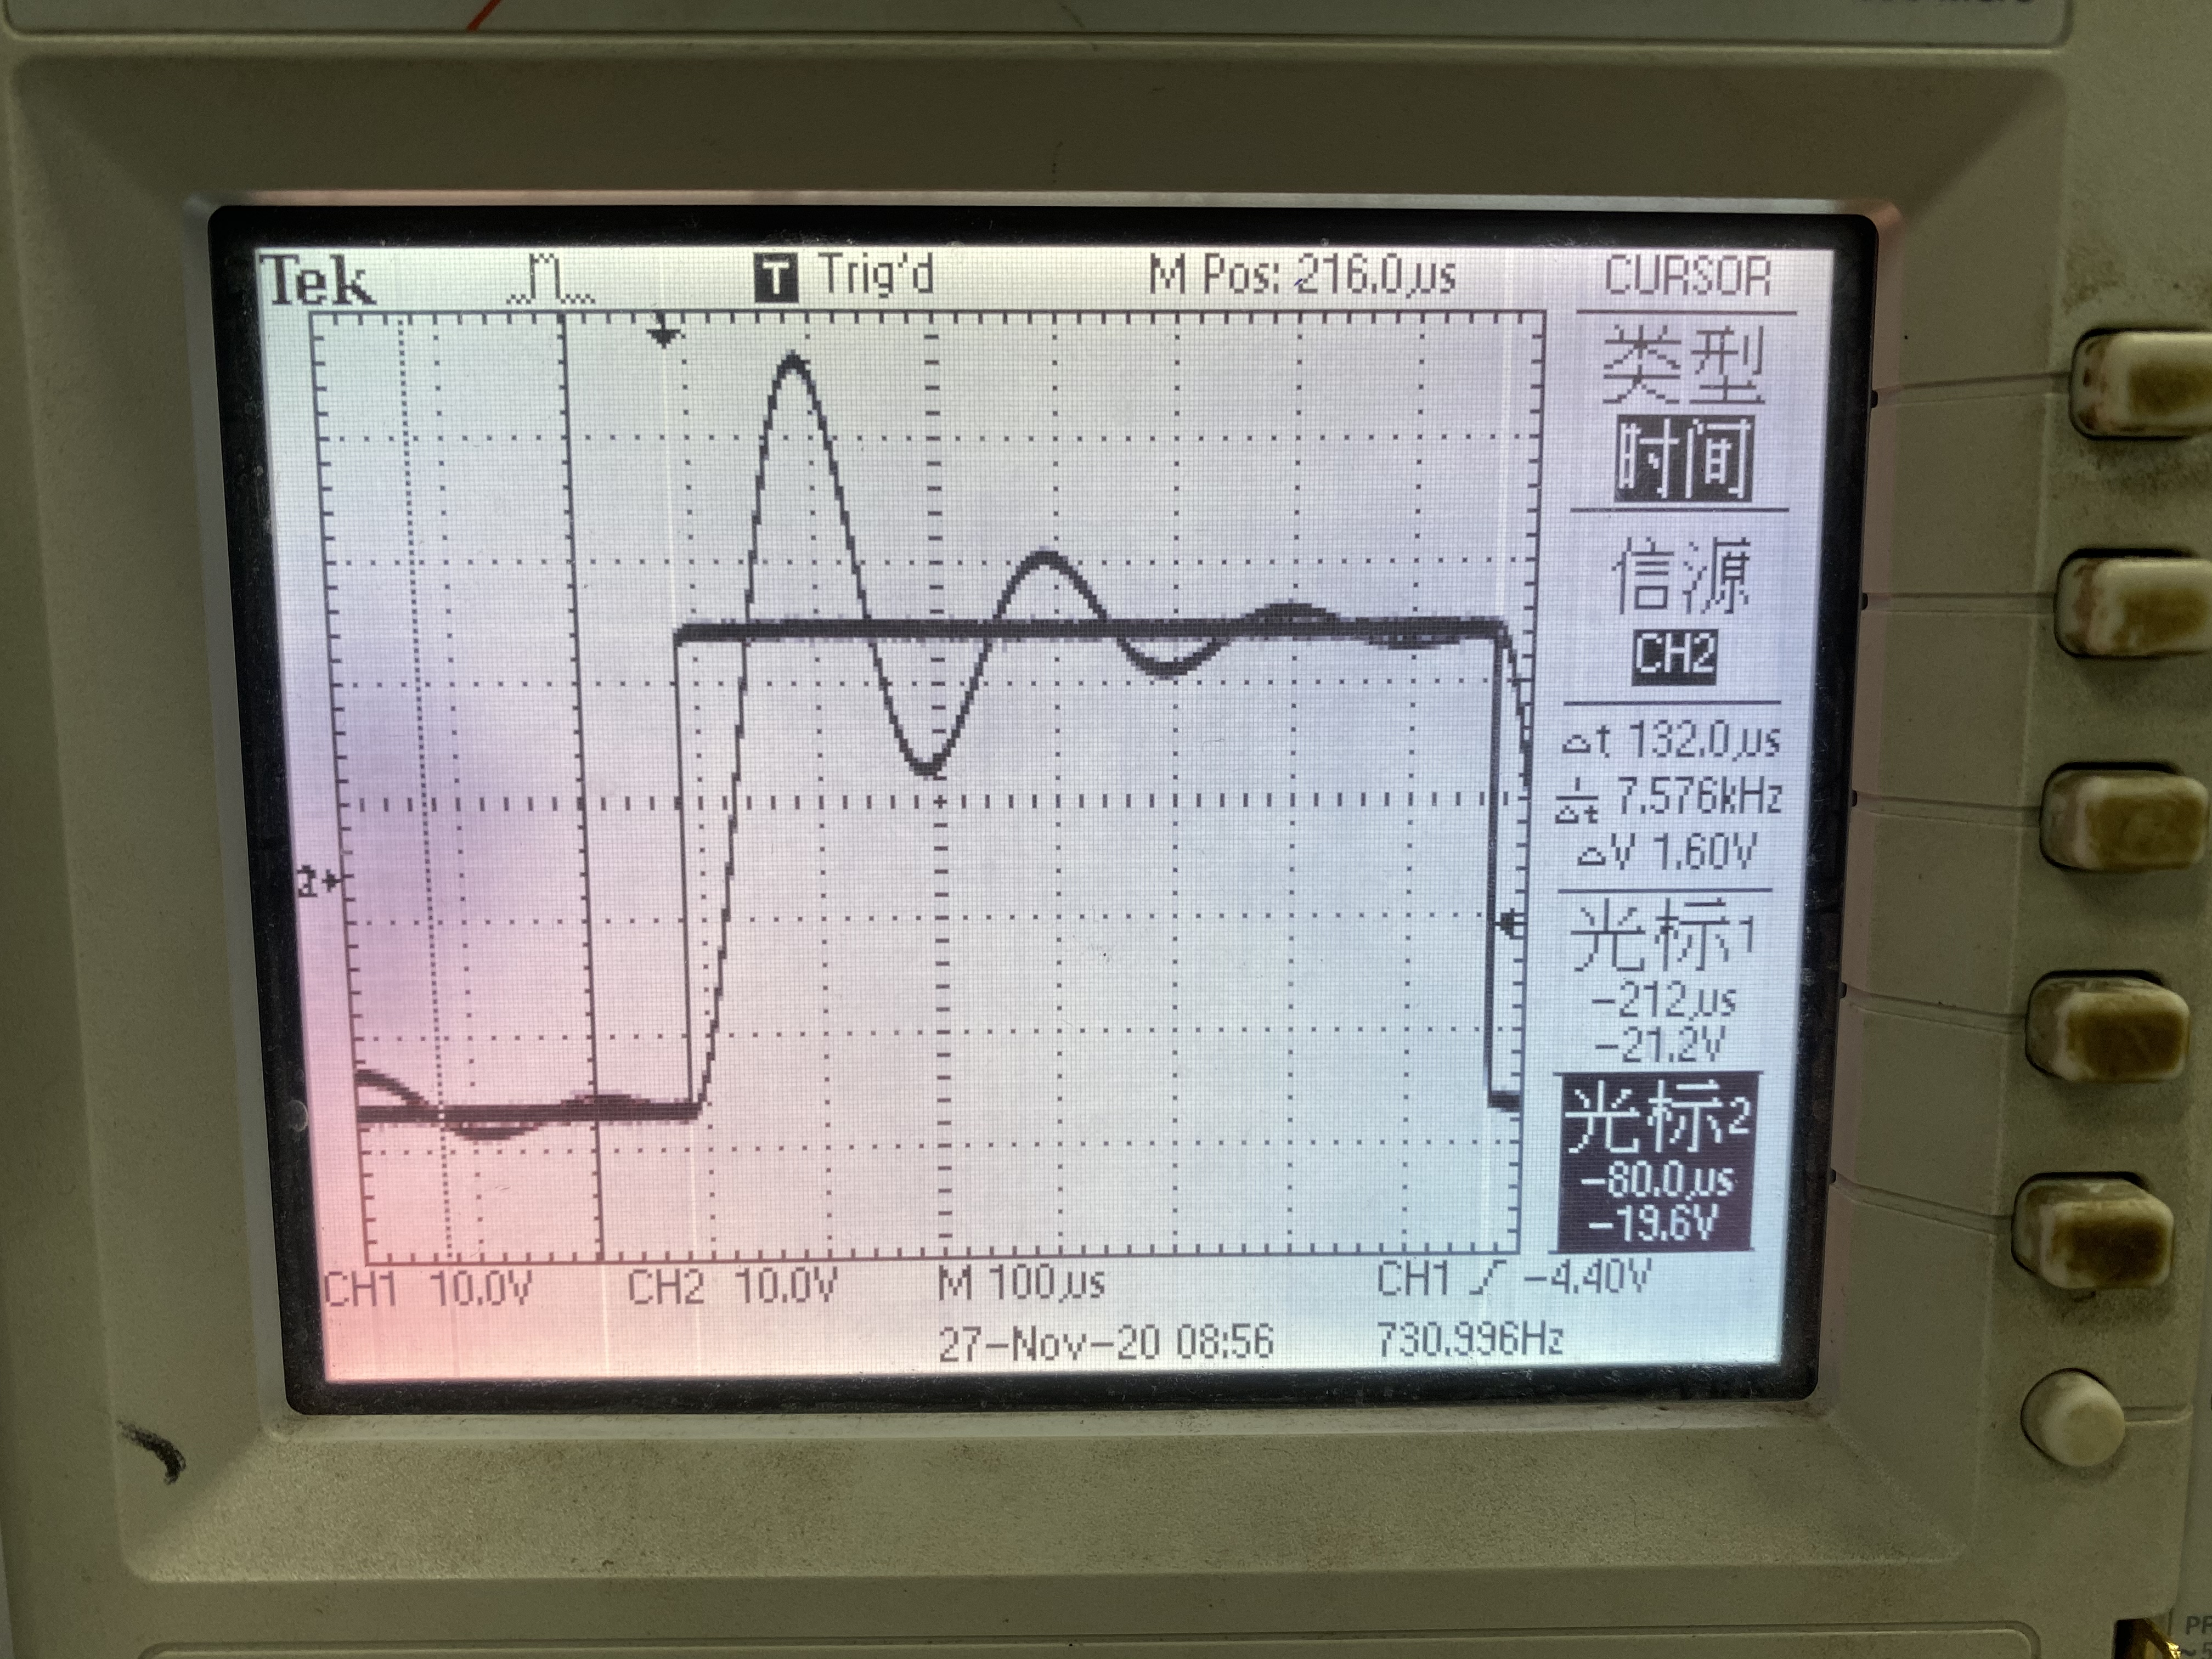
\includegraphics[width=6cm]{underdamp.jpg}
        \caption{Under-damped regime of RLC circuit}
    \end{minipage}  
    \begin{minipage}{0.49\linewidth}
        \centering
        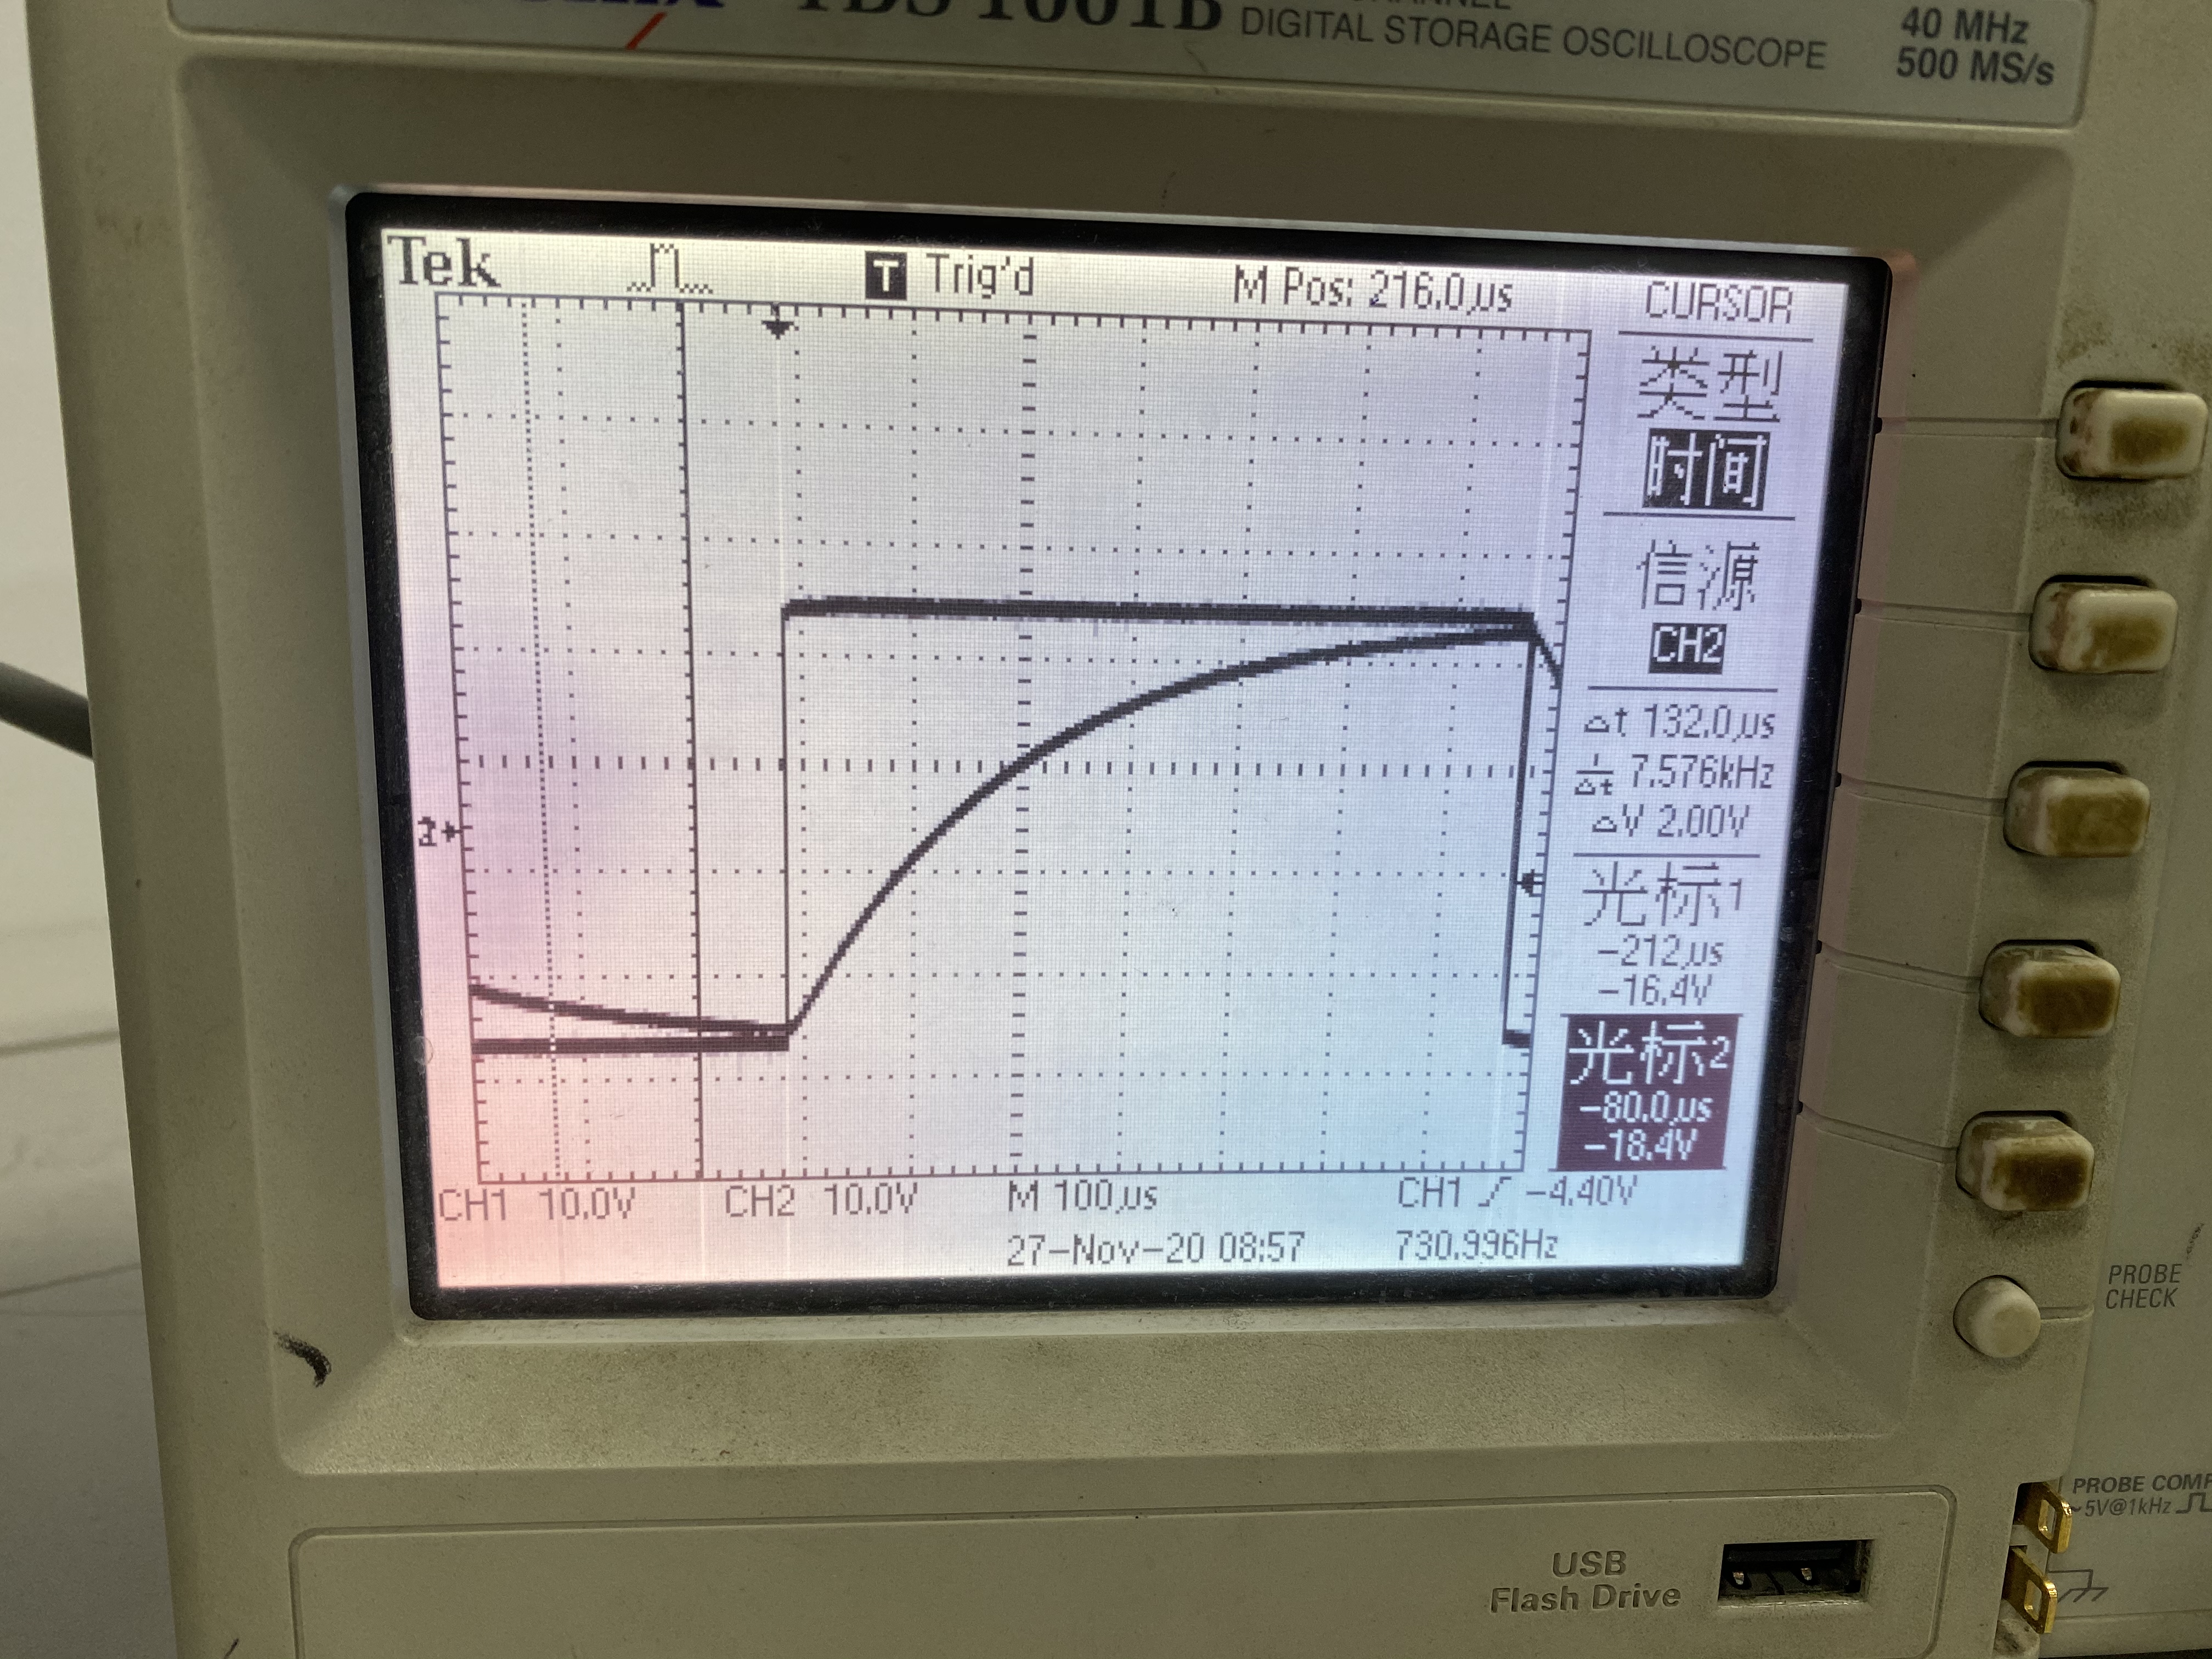
\includegraphics[width=6cm]{overdamp.jpg}
        \caption{Over-damped regime of RLC circuit}
    \end{minipage} 
\end{figure}

\begin{figure}[H]
    \centering
    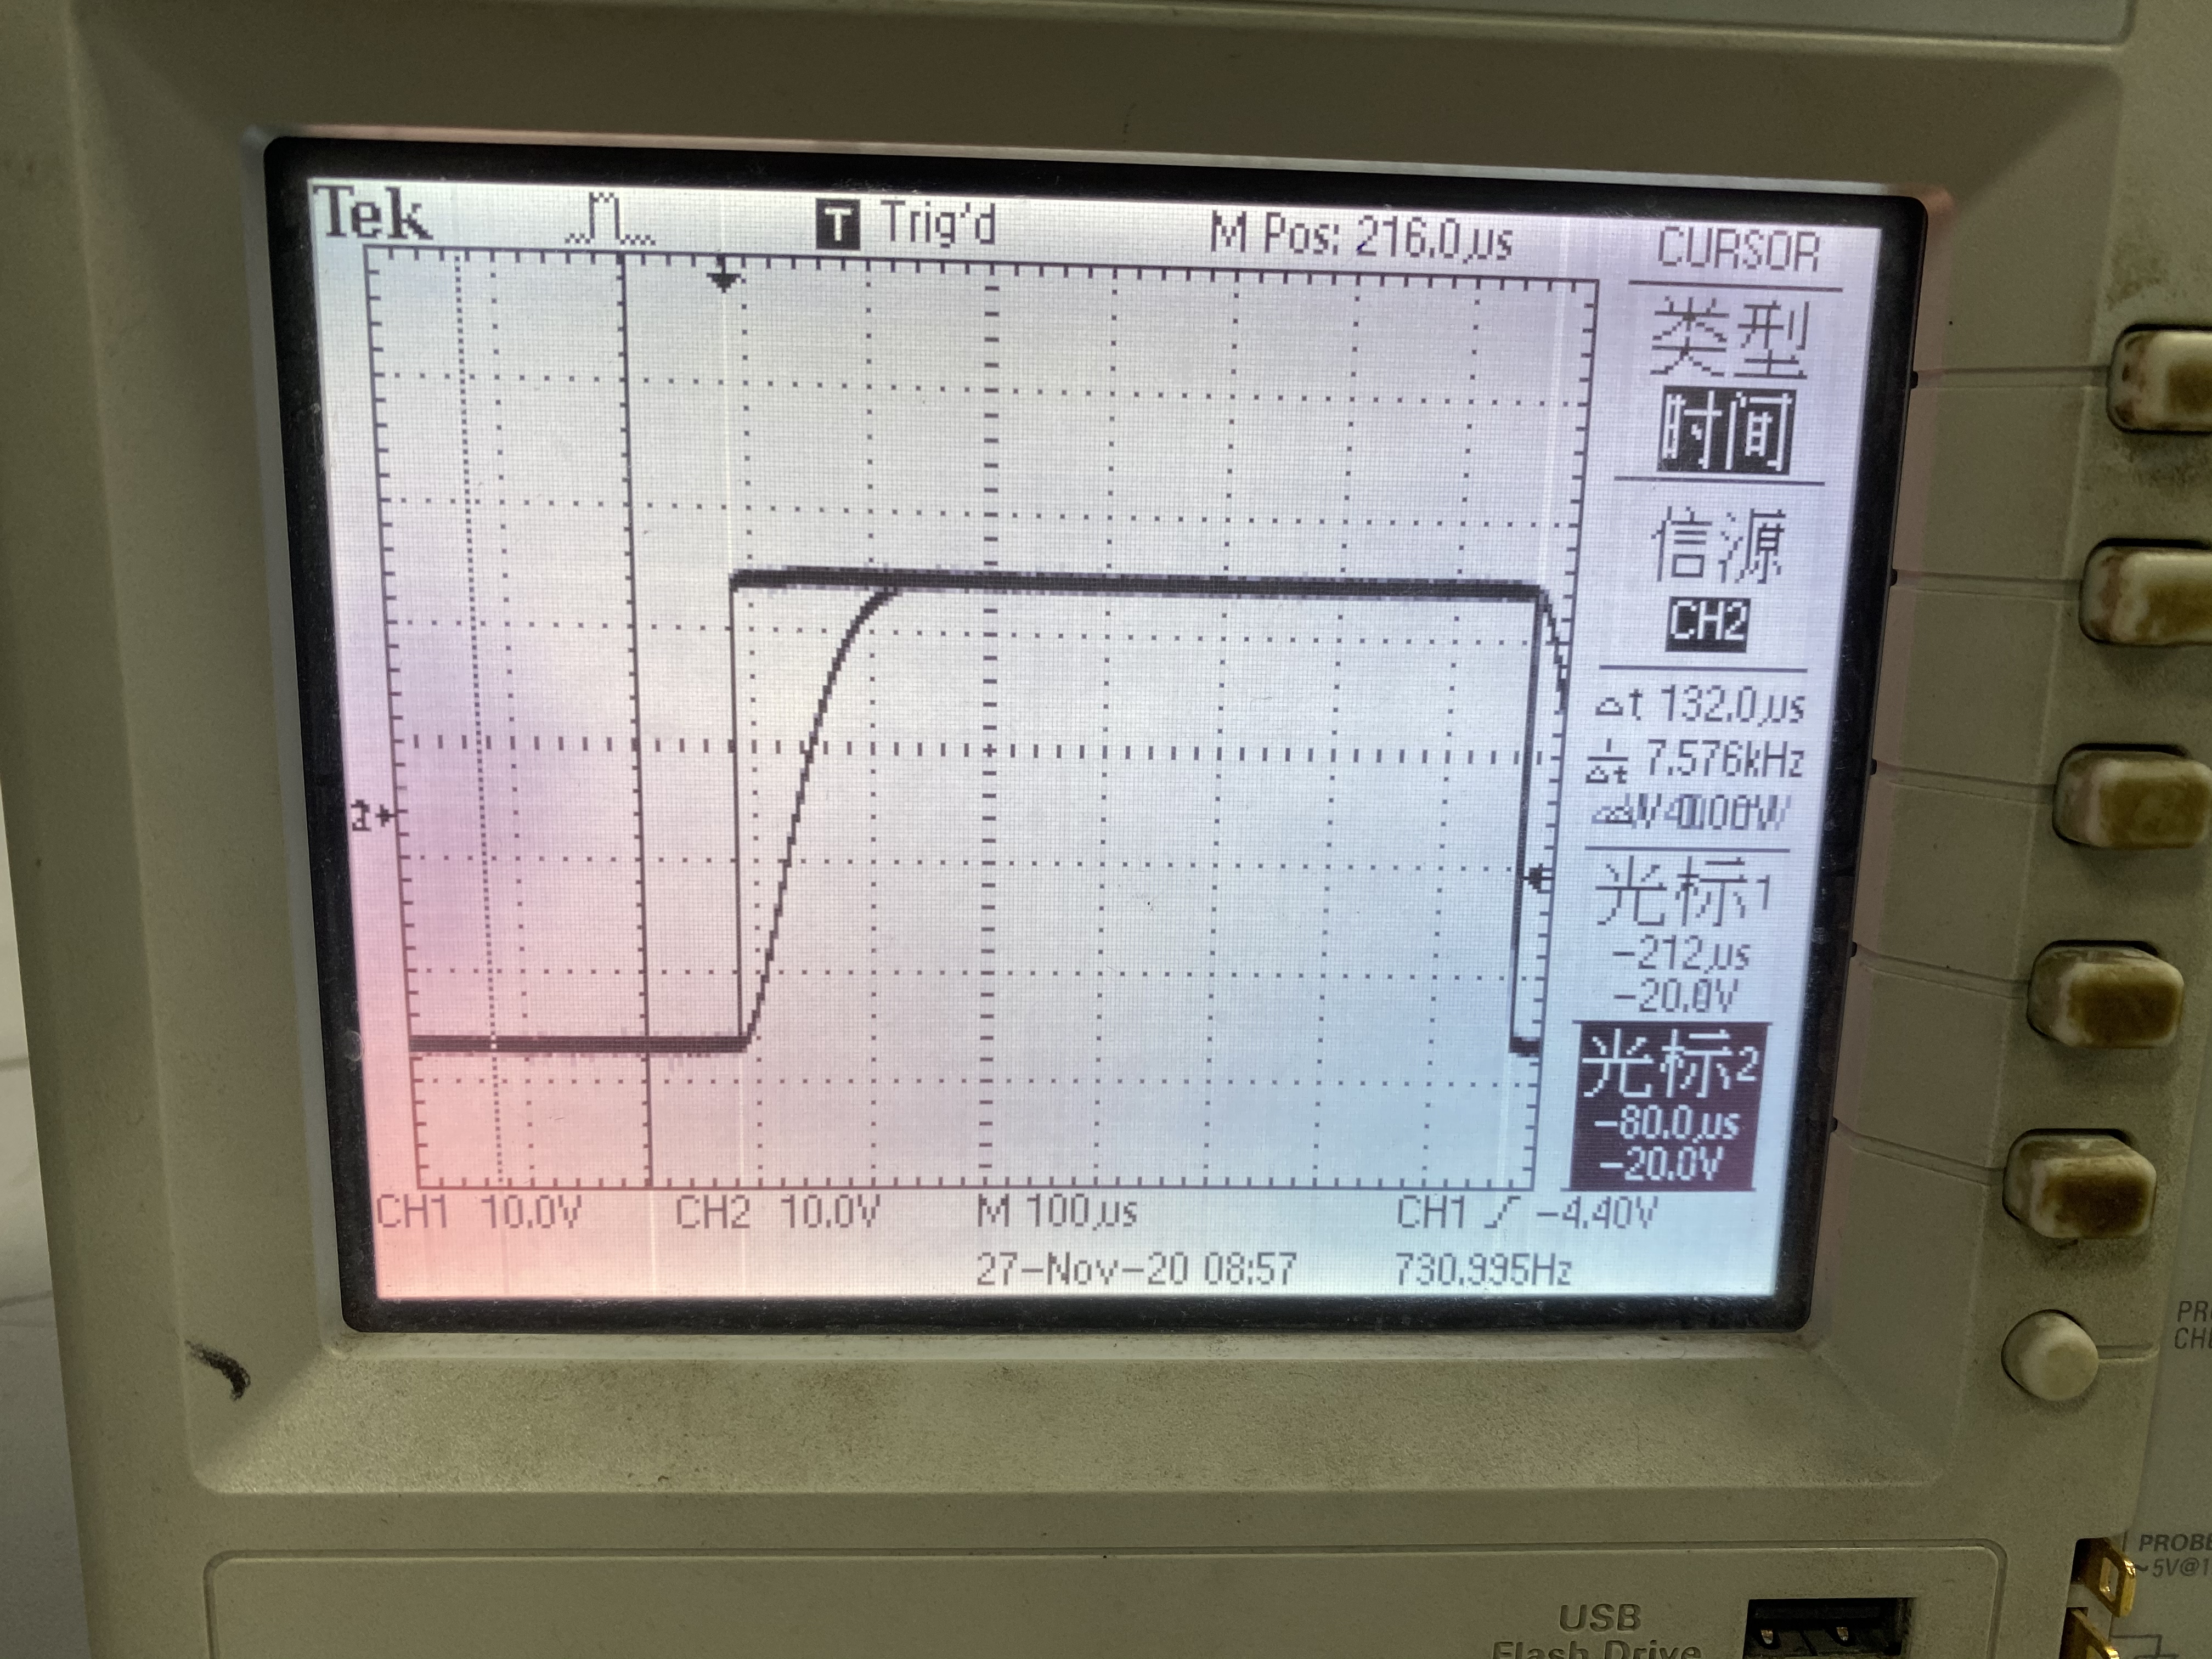
\includegraphics[width=7cm]{criticaldamp.jpg}
    \caption{Critically-damped rigime of RLC circuit}
\end{figure}

We than calculate the time constant $\tau_{exp}$:
$$\tau_{exp}=\frac{T_{1/2}}{\beta t}=\frac{52.00}{1.68}=30.952\pm0.006\mu s=30.952\pm0.006 [\times 10^{-6}]s$$

Theoretically, the time constant ${\tau}_{theo}$ should be:
$${\tau}_{theo}=\sqrt{LC}=\sqrt{0.01\times 99.6\times 10^{-9}}=31.560[\times 10^{-6}]s$$

The relative error is:
$$u_r==\frac{\tau_{exp}-\tau_{theo}}{\tau_{theo}}=\frac{30.952-31.560}{31.560}=-1.93\%$$

\subsection{RLC resonant circuit}
\begin{table}[H]
    \centering
    \begin{tabular}{|c|c|}
    \hline
    Quantities             & Value              \\ \hline
    R{[}$\Omega${]}        & 101.09$\pm$0.01    \\ \hline
    C{[}nf{]}              & 99.6$\pm$0.1       \\ \hline
    L{[}H{]}              & 0.01       \\ \hline
    $\mathcal{E}${[}Vpp{]} & 4.000$\pm$0.001    \\ \hline
    $f_0${[}Hz{]}          & 5040.000 $\pm$0.001    \\ \hline
    \end{tabular}
    \caption{Measurement Data for RLC Resonant circuit}
\end{table}
\subsubsection{Relationship between $\frac{I}{I_m}$ and $\frac{f}{f_0}$}
\begin{table}[H]
    \centering
    \begin{tabular}{|c|c|c|c|c|c|c|}
    \hline
    U[V]     & $u_U$[v]    & f[Hz]$\pm$0.001[Hz]         & f/$f_0$      & $u_{f/f_0}$     & I/$I_m$   & $u_{I/I_m}$  \\ \hline
    0.400 & 0.002 & 540.000   & 0.1071429 & 0.0000002 & 0.1000 & 0.0005 \\ \hline
    0.800 & 0.002 & 1740.000  & 0.3452381  & 0.0000002  & 0.2000 & 0.0005 \\ \hline
    1.24  & 0.02  & 2740.000  & 0.5436508  & 0.0000002  & 0.310  & 0.005  \\ \hline
    1.64  & 0.02  & 3340.000  & 0.6626984  & 0.0000002  & 0.410  & 0.005  \\ \hline
    1.96  & 0.02  & 3640.000  & 0.7222222  & 0.0000002  & 0.490  & 0.006  \\ \hline
    2.40  & 0.02  & 3940.000  & 0.781746  & 0.0000003  & 0.600  & 0.0060  \\ \hline
    2.72  & 0.02  & 4140.000  & 0.8214286  & 0.0000003  & 0.680  & 0.006  \\ \hline
    3.04  & 0.02  & 4340.000  & 0.8611111  & 0.0000003  & 0.760  & 0.006  \\ \hline
    3.44  & 0.02  & 4540.000  & 0.9007937  & 0.0000003  & 0.860  & 0.007  \\ \hline
    3.76  & 0.02  & 4740.000  & 0.9404762  & 0.0000003  & 0.940  & 0.007  \\ \hline
    4.00  & 0.02  & 5040.000  & 1.0000000  & 0.0000003  & 1.000  & 0.007  \\ \hline
    3.76  & 0.02  & 5340.000  & 1.0595238  & 0.0000003  & 0.940  & 0.007  \\ \hline
    3.56  & 0.02  & 5440.000  & 1.0793651  & 0.0000003  & 0.890  & 0.007  \\ \hline
    3.16  & 0.02  & 5740.000  & 1.1388889  & 0.0000003  & 0.790  & 0.006  \\ \hline
    2.72  & 0.02  & 6040.000  & 1.1984127  & 0.0000003  & 0.680  & 0.006  \\ \hline
    2.40  & 0.02  & 6340.000  & 1.2579365  & 0.0000003  & 0.600  & 0.006  \\ \hline
    1.96  & 0.02  & 6840.000  & 1.3571429  & 0.0000003  & 0.490  & 0.006  \\ \hline
    1.64  & 0.02  & 7640.000  & 1.5158730  & 0.0000004  & 0.410  & 0.005  \\ \hline
    1.24  & 0.02  & 9040.000  & 1.7936508  & 0.0000004  & 0.310  & 0.005  \\ \hline
    0.800 & 0.002 & 13340.000 & 2.6468254  & 0.0000006  & 0.2000 & 0.0005 \\ \hline
    0.560 & 0.002 & 20940.000 & 4.1547619   & 0.0000008   & 0.1400 & 0.0005 \\ \hline
    \end{tabular}
    \caption{Relation between I/$I_m$ and f/$f_0$}
\end{table}

\begin{figure}[H]
    \centering
    \includegraphics[width=9cm]{iimff0.png}
    \caption{Relation between I/$I_m$ and f/$f_0$}
\end{figure}

\subsubsection{Phase Shift}
$$\varphi_{theo}={tan}^{-1}{(}\frac{2\pi fL-\frac{1}{2\pi fC}}{R})~~~~~~\varphi_{exp}={cos}^{-1}{(}\frac{U_R}{U_m})$$

\begin{table}[H]
    \centering
    \begin{tabular}{|c|c|c|c|c|c|}
    \hline
     f/$f_0$ & $u_{f/f_0}$ & $\varphi_{ex}$  & $u_{\varphi_{ex}}$ & $\varphi_{theo}$  &  $u_{\varphi_{theo}}$ \\ \hline
    0.1071429 & 0.0000002 & -1.4106 & 0.0005 & -1.536252  & 0.000003  \\ \hline
    0.3452381  & 0.0000002  & -1.3694 & 0.0005 & -1.446488  & 0.000012  \\ \hline
    0.5436508  & 0.0000002  & -1.256 & 0.006 & -1.32964   & 0.00002   \\ \hline
    0.6626984  & 0.0000002  & -1.148 & 0.006 & -1.21079   & 0.00003   \\ \hline
    0.7222222  & 0.0000002  & -1.059 & 0.006 & -1.22688   & 0.00004   \\ \hline
    0.7817460  & 0.0000003  & -0.927 & 0.007 & -1.00165   & 0.00004   \\ \hline
    0.8214286  & 0.0000003  & -0.823 & 0.008 & -0.89408   & 0.00005   \\ \hline
    0.8611111  & 0.0000003  & -0.707 & 0.010 & -0.75697   & 0.00005   \\ \hline
    0.9007937  & 0.0000003  & -0.536 & 0.013 & -0.58333   & 0.00005   \\ \hline
    0.9404762  & 0.0000003  & -0.35  & 0.02  & -0.37074   & 0.00003   \\ \hline
    1.0000000  & 0.0000003  & 0      & Inf   & -0.0037519 & 0.0000013 \\ \hline
    1.0595238  & 0.0000003  & 0.35   & 0.02  & 0.34459    & 0.00003   \\ \hline
    1.0793651  & 0.0000003  & 0.473  & 0.015 & 0.44384    & 0.00004   \\ \hline
    1.1388889  & 0.0000003  & 0.660  & 0.010 & 0.68310    & 0.00005   \\ \hline
    1.1984127  & 0.0000003 & 0.823  & 0.008 & 0.84944    & 0.00005   \\ \hline
    1.2579365  & 0.0000003  & 0.927  & 0.007 & 0.96619    & 0.00005   \\ \hline
    1.3571429  & 0.0000003  & 1.059  & 0.006 & 1.09493    & 0.00004   \\ \hline
    1.5158730  & 0.0000004  & 1.148  & 0.006 & 1.21361    & 0.00003   \\ \hline
    1.7936508  & 0.0000004  & 1.256  & 0.006 & 1.31794    & 0.00002   \\ \hline
    2.6468254  & 0.0000006  & 1.3694  & 0.0005 & 1.430998   & 0.000014  \\ \hline
    4.1547619   & 0.0000008   & 1.4303  & 0.0005 & 1.489412   & 0.000008  \\ \hline
    \end{tabular}
    \caption{Calculation result of phase shift}
\end{table}

\begin{figure}[H]
    \centering
    \includegraphics[width=9cm]{phitheo.png}
    \caption{$\varphi_{theo}$ vs $\frac{f}{f_0}$}
\end{figure}

\begin{figure}[H]
    \centering
    \includegraphics[width=9cm]{phiex.png}
    \caption{$\varphi_{ex}$ vs $\frac{f}{f_0}$}
\end{figure}
The theoretical resonate frequency
$$f_{0,theo}=\frac{1}{2\pi\sqrt{LC}}=\frac{1}{2\pi\sqrt{0.01\times99.6\times{10}^{-9}}}=5043[Hz]\pm 3[Hz]$$
$$u_r==\frac{f_0-f_{0,theo}}{f_{0,theo}}=\frac{5040.000-5043}{5043}=-0.06\%$$

\subsection{Quality factor}
$$Q_{theo}=\frac{\sqrt{LC}}{RC}=\frac{\sqrt{0.01\times99.6\times{10}^{-9}}}{101.09\times99.6\times{10}^{-9}}=3.1344\pm 0.0003$$

when $I(f_1) = I(f_2) = Im/\sqrt{2}$,$U_R(f_1)=U_R(f_2)=\frac{U_m}{\sqrt{2}}=\frac{4.00}{\sqrt{2}}=2.83Vpp$
The closet frequency is $f_1$=4140Hz $f_2$=6040Hz. 
$$Q_{exp}=\frac{f_0}{f_2-f_1}=\frac{5040}{6040-4140}=1.438\pm1\times{10}^{-6}=2.652632\pm 0.000006$$

$$r=\frac{Q_{exp}-Q_{theo}}{Q_{theo}}=\frac{2.6526-3.1344}{3.1344}=-15.37\%$$


\section{Conclusions and Discussions}

In this lab, we can achieve the following goals and significances:
\begin{itemize}
    \item Understand the physics of alternating-current circuits, especially the dynamic process in RC, RL, and RLC series circuits.
    \item Study methods for the amplitude-frequency and the phase-frequency characteristics
    \item Find the resonance frequency and quality factor of RLC circuit.
\end{itemize}

In RC circuit, the time constant is found: $\tau_{exp}=51.94\pm0.01[\mu s]$ and $\tau_{theo}=46.00\pm0.01[\mu s]$ The relative error is 12.9\% \par

In RL circuit, the time constant is found: ${\tau}_{exp}=100.99\pm0.01[\mu s]$ and ${\tau}_{theo}=100.00\pm0.01[\mu s]$ The relative error is 0.99\% \par 

In RLC circuit, the time constant is found: ${\tau}_{exp}=83.33\pm0.06[\mu s]$ and ${\tau}_{theo}=67.86\pm\mathrm{0.007}[\mu s]$ The relative error is 22.8\% \par 
When $f=f_0$, the circuit reaches resonance and I reaches its maximum. Far from $f_0$, I becomes smaller and the experimental figure match the theoretical one.\par 
We can find the phase shift increase in Fig.13 and Fig.14. Theoretically, when f=$f_0$, the phase shift is 0. When f<$f_0$, the phase shift is negative. When f>$f_0$, the phase shift is positive. The phase shift is close to $\pi/2$ if f/$f_0$ is really small or big. \par 
The resonant frequency is found at $f_0=2300.000\pm0.001Hz$. Compared with the theoretical value: $f_{0,theo}=2345.3\pm0.3Hz$, the relative error of $f_0$ is -1.93\%. \par 
The quality factor is found: $Q_{theo}=1.472\pm0.0002\text{ and }Q_{exp}=1.438\pm1\times{10}^{-6}$
The relative error is -2.31\%.\par 

The uncertainty may caused by the following reasons.
\begin{itemize}
    \item The large relative error of time constant may because of the inaccuracy while reading $T_{1/2}$. Since U cannot reach precisely half of $U_m$. 
	\item In RLC part, it's hard to determine the critically-damped simply by eyes.
	\item The oscilliscope may have resistance.
	\item The resistance may change because of rise of temperature.
	\item When calculating the experimental quality factor, we just take the closest values from $\frac{I_m}{\sqrt{2}}$ as $f_1$ and $f_2$ from our experimental data.
\end{itemize}

Change the resistor digitally to more precisely reach the critically-damped regime. Improve the accuracy of the equipment. Repeat the experiment of resonant series to find more precise $f_1$ and $f_2$. These may help us improve the accuracy.


\section{Reference} 
[1] Qin Tian, Feng Yaming, Gu Yichen, Mateusz Krzyzosiak. Physics Laboratory VP241 Ex-
ercise 5: RC, RL, and RLC Circuits.


\begin{description}
    \item[]   
\end{description}

{\LARGE\textbf{APPENDIX}}
\setcounter{section}{0}
\renewcommand\thesection{\Alph{section}}
\section{Data Sheet}


\end{document}